\documentclass{article}

\usepackage{graphicx}

\author{Ipatie Daniel și Lorena Maria Vitan}
\title{IMAGISTICA PRIN REZONANȚĂ MAGNETICĂ NUCLEARĂ }
\date{}


\begin{document}
    \maketitle

    \section{Prezentare generală}

    Tema site-ului este "IMAGISTICA PRIN REZONANȚĂ MAGNETICĂ NUCLEARĂ", acesta a fost făcut folosind framework-ul "Vue.JS" și librăria MagicScroll pentru a anima apariția datelor de pe site.

    \section{Programe Folosite}

    \begin{itemize}
        
        \item NeoVim - Editor Text
        \item Vue.JS - Framework Principal
        \item MagicScroll - Librarie pentru animație
        \item Netlify - Serviciu de deployment
        \item GitHub - Sistem de version control
        \item NPM - Manager de packete și sistem de compilare
        \item {\LaTeX}  - Sistemul de scriere pentru documentație
        
    \end{itemize}


    \subsection{Motive pentru alegeri}

    \subsubsection{Vue.JS}
    Am ales framework-ul Vue.JS deoarece oferă o flexibilitate mai mare decât celelalte framework-uri disponibile și în același timp o continuitate a sintaxei.

    Angular.JS oferă o stabilitate mai mare decât Vue.JS dar în consecință sintaxa și module de a crea componente este puternic influențată de StrongTyped languages. Acesta find creat de către Google urmează filozofia impusă de către aceștia și nu permite ambiguitate din punct de vedere al codului și din această cauză librăriile disponibile sunt scrise într-un mod bizar pentru un framework.

    React.JS este un framework dezvoltat de către Facebook și prezintă mai multă flexibilitate decât Angular.JS dar sacrifică continuitatea de sintaxă și de logică, acesta este cel mai popular framework de pe piața de muncă deoarece prezintă un suport foarte bun pentru dispozitivile Android și Apple.

    \subsection{NeoVim}

    Prefer NeoVim ca editor de text deoarece este o versiune îmbunătățită a programului vim care la rândul lui este succesorul editorului vi. Acesta oferă utilizatorului abilitatea de a-și crea propriile comenzi și scurături pentru a-și crea o experienț unică pentru propriile nevoi.

    NeoVim spre deosebire de alte programe de editare cum ar fi Visual Studio Code sau Sublime Text prezintă abilitatea de a crea macro-uri, adică de a înregistra comenzi succesive pentru executare repetată, astfel având o diversificare mult mai mare neavând nevoie de editare constantă pentru a crea o comandă folosită pentru o situație specifică ci o poți face pe loc.

    \subsection{Netlify}

    Am ales serviciul oferit de Netlify deoarece spre deosebire de alte servici precum a2hosting, heroku deoarece are posibilitatea de a menține aplicați pe internet pentru un timp indefinit cu condiția ca aceasta să nu depășească un anumit bandwith alocat.

    Acesta prezintă un sistem de integrare alocat de către GitHub pentru a face un deployment continu și sigur pentru a nu pierde progres raportează erori la build-ul site-ului. Aceste permite și crearea de un "Custom Domain" care are sufixul ".netlify.app" acesta find un deranj minor aproape inexistent.

    \subsection{{\LaTeX}}

    {\LaTeX}  este un sistem de scriere al documentelor care permite configurare ușoară și exstinsă a documentelor de tip PDF pentru a crea documente și lucrări. Spre deosebire de Word, acest mod de scriere de documente permite crearea de comenzi și de funcții speciale pentru a personaliza procesul de scriere.

    \section{Descriere}

    Imagistica medicală a înregistrat un progres real odată cu introducerea RMN-ului ca tehnică imagistică de diagnostic. Principalele caracteristice ale acestei tehnici sunt neinvazivitatea și calitatea marea a imaginii. Scleroza multiplă, boală neurologicâ demielinizantă, este un exemplu relevant de aplicație a RMN-ului în studiul sistemului nervos central. 
 
    \subsection{GENEZA SEMNALULUI RMN}


    Metoda se bazează pe fenomenul fizic al rezonanței magnetice nucleare. 

    O imagine obținută traduce în semnale optice intensitatea semnalelor de radiofrecvență (RF) ale unor nuclei atomici din structuri anatomice examinate. 

    Metoda se bazeazâ pe proprietatea unor nuclei atomici, în special a celor de hidrogen (respectiv protonilor) de a realiza o mișcare de rotație în jurul propriului ax, adică de a avea un moment cinetic propriu, spinul nuclear.

    Rotația unei particule încărcate electric, cum este protonul, determinâ apariția unui câmp magnetic propriu orientat în sens opus câmpului electric.

    Această transformă fiecare nucleu într-un dipol magnetic, un magnet microscopic. (pic 2) 


\subsection{ETAPELE OBȚINERII IMAGINII PRIN REZONANȚĂ MAGNETICĂ (IRM)}


Obținerea imaginii prin aceste fenomen de rezonanță magneticâ cuprinde câteva momente distincte.

În condiții obișnuite, orientarea micromagneților reprezentați de nucleii atomici din structurile anatomice este întâmplătoare. (fig 2a)

Câmpurile magnetice individuale se neutralizeazâ reciproc, astfel că manifestările lor nu sunt decelabile.


\subsection{TREPTELE GENEZEI SEMNALULUI RMN}


Aplicarea unui câmp magnetic exterior foarte puternic produce alinierea lor în direcția acestuia 

Un impuls scrut RF determinâ intrare în rezonanță a nucleilor

Dupâ suprimarea impulsului RF, nucleii își continuâ oscilația, emițând o undâ de radiofrecvență decelabilâ.

Corpul uman este supus unui câmp magnetic exterior foarte puternic, care rămâne constant în timpul investigației și care produce alinierea în aceeași direcție a dipolilor magnetici nucleari.

Se aplică apoi o undă de radiofrecvență (RF), ceea ce determină rezonanța nucleilor. 

REZONANȚA este fenomenul de oscilație a unui sistem fizic, determinat de energia primită de la un alt sistem, cu care se află în legătură directă sau prin intermediul undelor și care oscilează cu o frecvență egală (sau apropiată) cu una din frecvențele cu care primul sistem este capabil să oscileze. 

Cu cât frecvența celui de al doilea sistem (furnizor de energie) este mai apropiată de frecvența posibilă a primului, amplitudinea oscilației actuia devine mai mare.

Unda de RF este apoi suprimată. Nucleii continuă să oscileze, emițând o undă de RF, care poate fi detectată ca semnal rezonant magnetic al nucleilor. 

Recepția semnalului este posibilă prin faptul că unda respectivă induce un curent electric într-o bobină constituită în acest scop.

Acest semnal este transmis unui computer, care îl transformă, prin prelucrare digitală, în semnale optice elementare (pixeli).

Pe calea unei matrice, suma acestor semnale, transcrise într-o anumită ordine, compune imaginea sintetică finală.

Valoarea sau intensitatea pixelului (adică treapta de gri atribuită pe scara de nuanțe între alb și negru) este proporționalâ cu intensitatea semnalului ce provine din nucleii rezonanți aparținând unui volum bine determinat, voxelul.

în afara densității protonilor în voxelul respectiv, această valoare mai depinde de doi determinanți temporali, etichetați T1 și T2. 

\subsection{DIFERENȚĂ FAȚĂ DE ALTE PROCEDURI IMAGISTICE }

1. Structurile examinate interacționează cu un factor fizic exterior ( radiația X, ultrasunetele), atenuându-l sau reflectându-l, în IRM structurile sunt stimulate pentru a produce ele însele semnale utilizabile în producerea unei imagini. 

2. Formarea imaginii implică participarea nucleilor atomici din mediul investigat și nu a straturilor electronice ale atomilor ( ca în cazul tehnicii radiodiagnostic). 

3. Ca și ultrasonografia, IRM recurge la un factor fizic neionizant, lipsit de nocivitate, aparținând metodelor de exploarare neinvazive. 


\subsection{TIMPII FIZICI DE RELAXARE ( T1 și T2)}

Durata semnalului RMN, este impusă de două procese fizice, care acționează în sens limitativ : 

Revenirea nucleilor oscilanți la poziția lor inițială ; 

aceasta se însoțește de scăderea exponențială în timp a amplitudinii semnalului ; are ca substrat transferul de energie de la nucleii în precesie către moleculele mari ale vecinătății ;

aceste molecule formează în jurul nucleilor rezonanți o veritabilă rețea, căreia îi este cedată energia dobândită de nucleii respectivi prin pulsul RF. 

Durata semnalului restrănsâ prin interacția nucleilor rezonanți (posesori de spin) cu rețeaua structurilor moleculare înconjurătoare este denumită timp de relaxare spin-rețea sau constantă de scădere exponențială T!.

Un alt termen folosit în exprimarea acestui timp este timpul de relaxare longitudinală .


\subsection{SUBSTRATUL BIOLOGIC}


Semnalele provin de la protonii corpului uman examinat; însă nu toți participă la producerea lor ;

Nucleii implicați în apariția semnalelor sunt din apa celulară, care constituie cea mai mare proporție a protonilor din corpul uman și din lipide . 

Este de așteptat ca starea apei tisulare să determine, pe lângă intensitatea semnalelor respective și valorile T1 și T2

Se acceptă așa-numitul concept al apei libere și legate care poate constitui o explicație satisfăcătoare pentru T1.

În celule și țesuturi, o proporție din apă este legată la suprafața proteinelor ; mișcarea de precesie a nucleilor de hidrogen va fi rapid încetinită datorită vecinătății moleculelor mari, ceea ce va avea ca rezultat un T1 scurt



\subsection{PRODUCEREA IMAGINII }



Imaginea RMN rezultă prin alăturarea unui număr variabil de pixeli, a căror valoare este determinată de amplitudinea fiecăruia din semnalele cu originea într-o unitate de volum.

Aceste volume elementare se găsesc dispuse într-un plan de secțiune prin corpul uman, astfel încât, ca și în cazul CT, imaginea RMN este de fapt o imagine tomografică realizată în planul respectiv

Pentru ca ea să capete semnificația dorită, nu este suficient ca semnalele RMN provenite din fiecare volum elementar examinat să fie recepționate ; aceste semnale trebuie să cuprindă și informații cu privire la poziția exactă în spațiu a volumelor respective

Poziția pixelilor în matrice trebuie să realizeze în ansamblu o veritabilă hartă a secțiunii anatomice

Acest deziderat creează în cazul IRM probleme tehnice complexe



\subsection{GRADIENȚII MAGNETICI}

Aceste câmpuri poartă denumirea de gradienți magnetici și se aplică pe una din coordonatele spațiale x, y sau z, de unde și denumirea de câmpuri de gradient liniar.

\subsection{EXCITAȚIA SELECTIVĂ }


Corpul uman este plasat în câmpul magnetic exterior foarte puternic.

Pentru obținerea excitației selective se aplică în aceeași direcție spațială un câmp-gradient mult mai slab, care variază de-a lungul pacientului, astfel încât este mai redus la extremitatea lui superioară și mai intens la cea inferioară. Rezultă un câmp magnetic total, care crește și el în același sens.

Tehnica excitației selective este aplicată pentru a alege planul ce va fi reprezentat în imagine. Poate fi aleasă o secțiune tomografică sagitală, utilizând un gradient dispus transversal, sau una frontală, cu un gradient orientat antero-posterior.


\subsection{ECHIPAMENTUL IRM}

3.1 Magnetul 


Este piesa centrală a instalației IRM ; el trebuie să producă un câmp magnetic extern, cât mai uniform, evitând pe cât posibl variațiile.


IRM realizează un foarte bun contrast între substanța albă și cea cenușie, imposibil de obținut prin altă metodă imagistică, ceea ce permite sesizarea unor procese patologice subtile, ce se produc la interfața acestora, de exemplu anomaliile de mielinizare ale copilului, scleroza multiplă și alte afecțiuni demielinizante.

De asemenea, alte procese patologice pot fi reprezentate în imagine, precum edemul, infarctul, hemoragiile cerebrale.

În cazul unor tumori cerebrale, diferențele între timpii de relaxare pe care le creează anumite variații histologice ( astrocitomul, meningiomul, metastazele) pot fi sugestive pentru natura acestora.

\subsection{INVESTIGAREA CREIERULUI ȘI STRUCTURILOR NERVOASE }

Scleroza multiplă (SM) este o entitate patologică neurologică invalidantă, frecventă în țările europene cu climă temperată. 

SM este o afecțiune inflamatorie ce implică sistemul imunitar, cu etiologie probabil virală, asociată unei susceptibilități genetice individuale. Nu s-a descoperit încă un agent responsabil, nu s-a nominalizat un factor ereditar implicat, deși s-au efectuat numeroase studii genetice. 

\section{Manualul de Programare}

\subsection{Principiul Vue.JS}

Sistemul de creare de site-uri Vue.JS are la baza sa o filozofie de componente și anume că fiecare element poate fi și ar trebuii să fie un component deoarece permite ca programatorul să aibă abilitatea de a modifica paginile web cu ușurință.

De asemenea și alte sisteme precum React.JS sau Angular.JS urmează o filozofie similară, dar diferența se află în modul de implementare al acestei filozofii, modul în care este implementat în vue permite o modalitate de citire mult mai ușoară și o structură de cod mult mai curată pentru programator.


\section{Exemplu de Vue.JS}
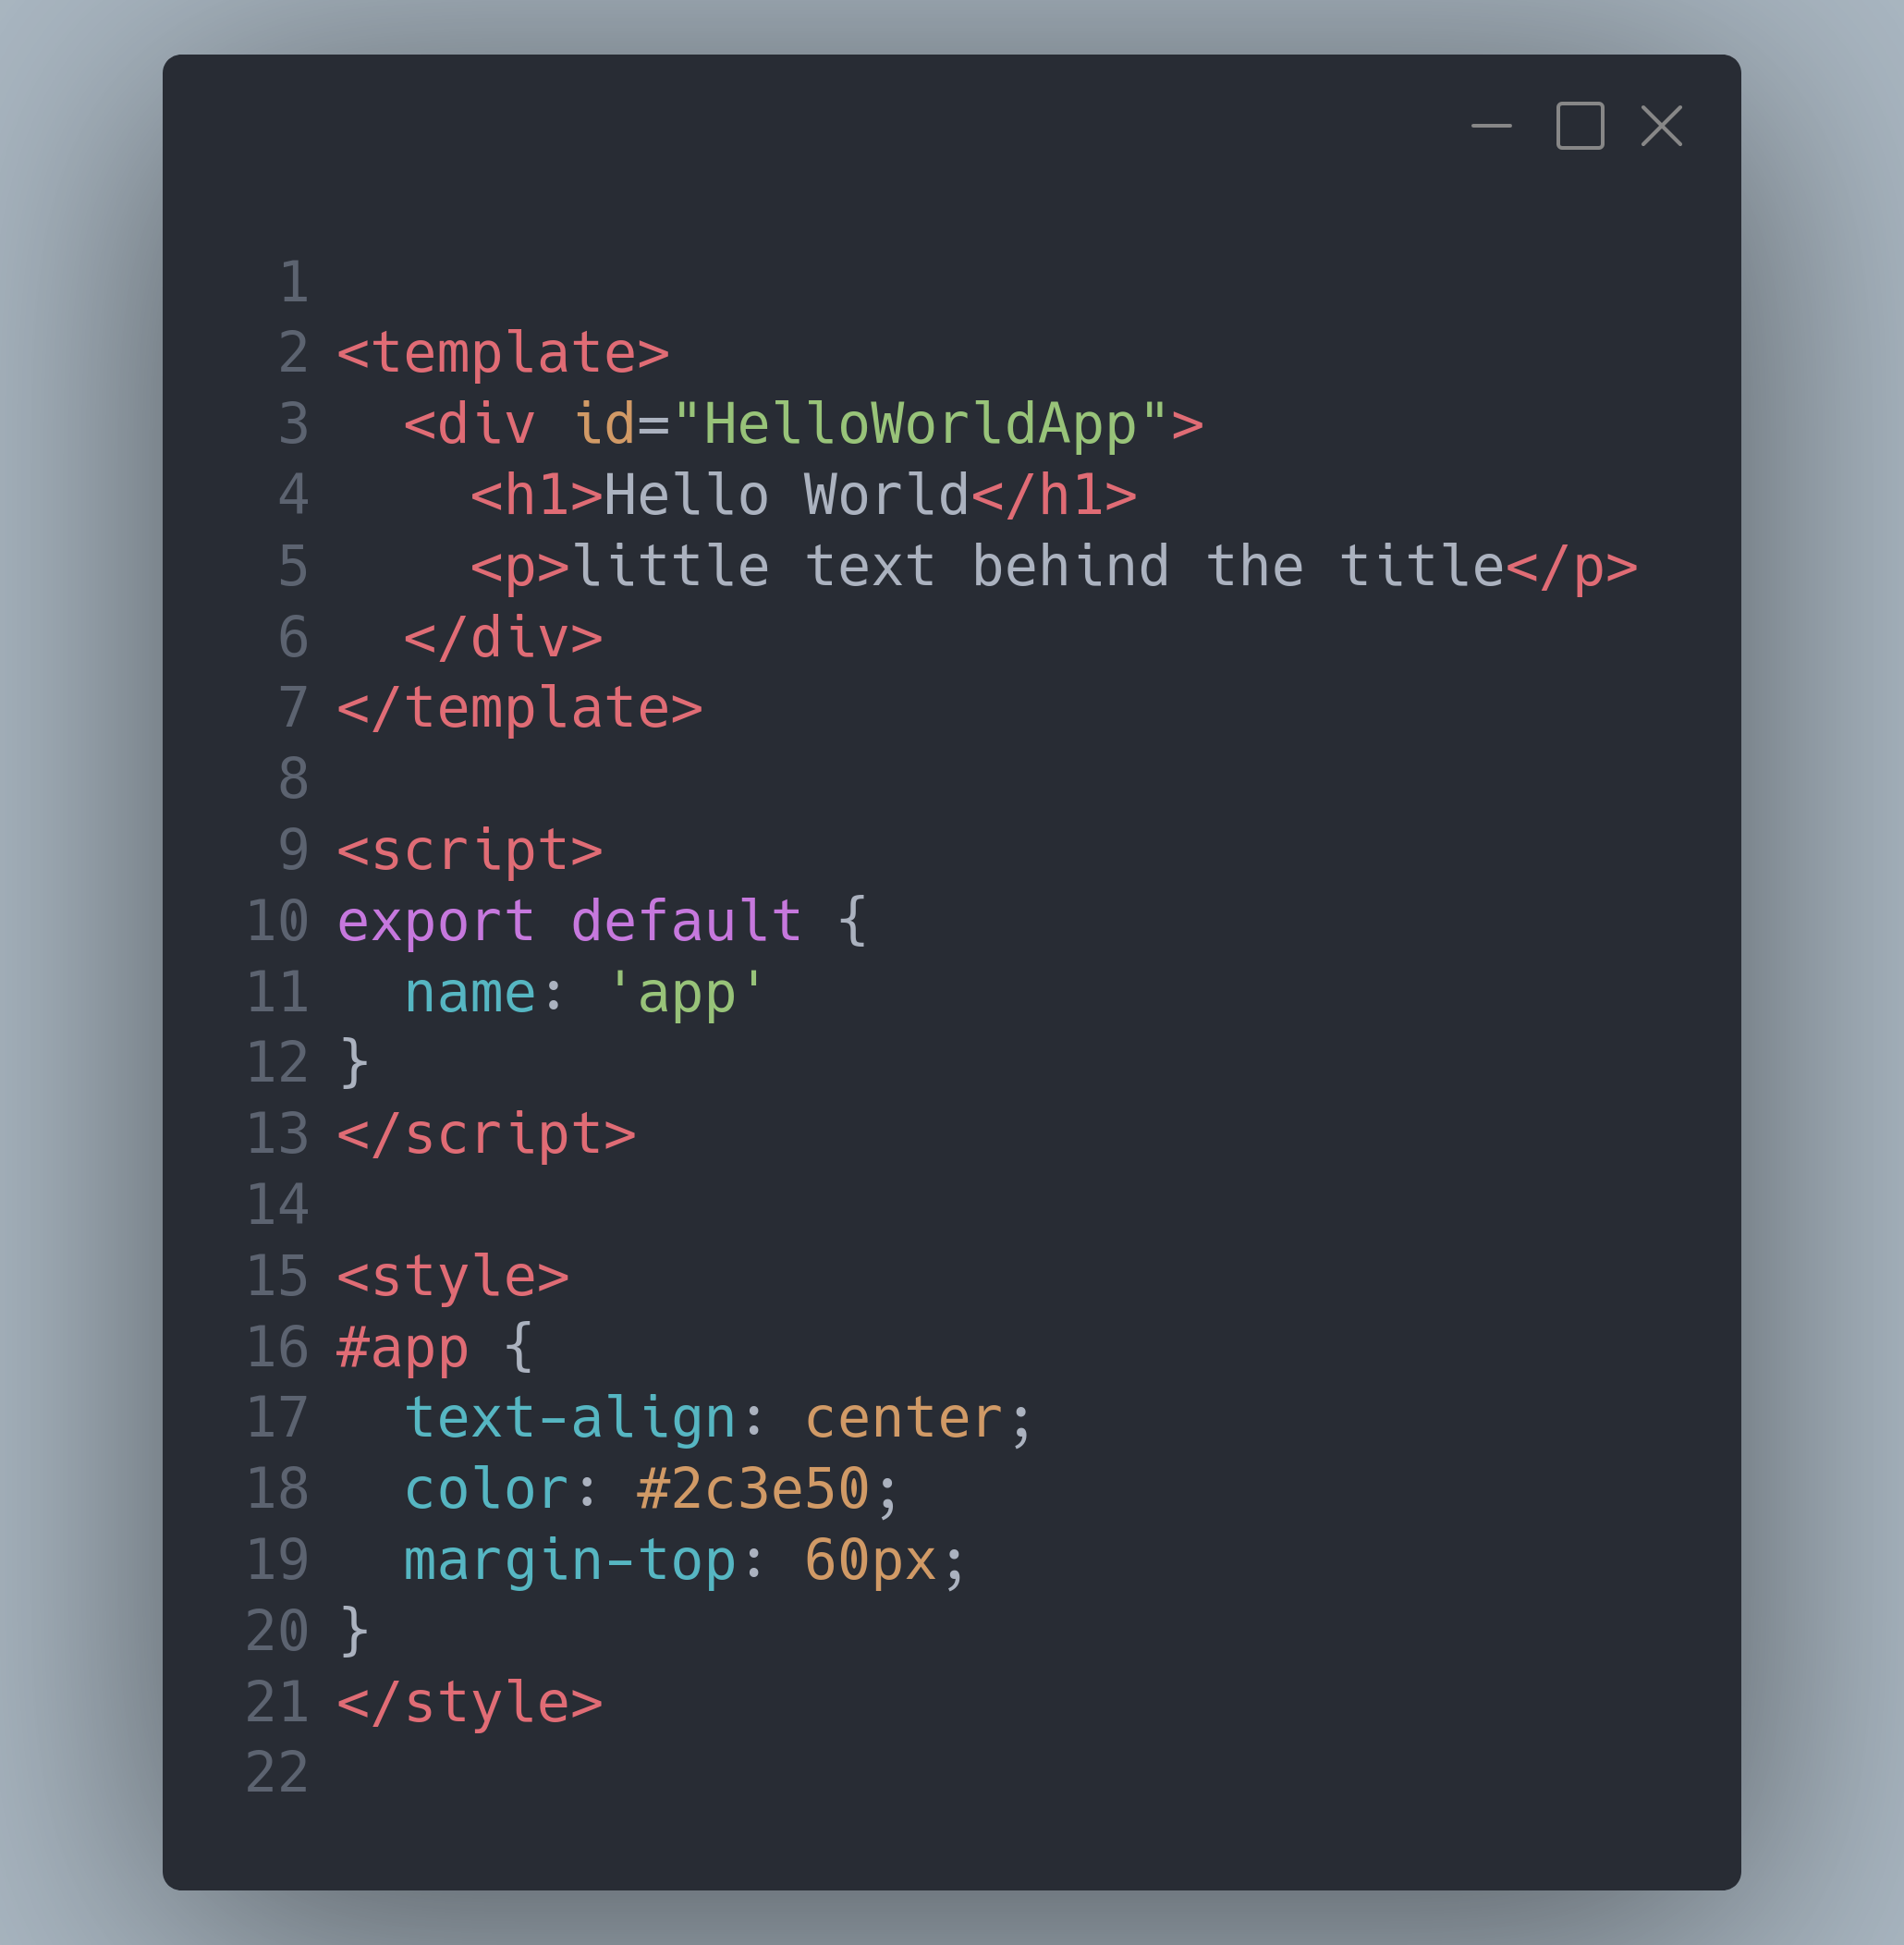
\includegraphics[width=\textwidth]{exampleVue1.png}

Acest exemplu de Vue.JS prezintă un component Hello World, după cum
se poate observa în imaginea de mai sus codul este împărțit în trei
părții, prima parte este înconjurată de $<template> </template>$ cea
ce înseamnă că face parte din sistemul de HTML Template pentru Vue,
partea ce se află între $<script> </script>$ are rolul de sistem
javaScript logic iar tagul de $<style> </style>$ prezintă sistemul de
compilare a fișierului css al componentului, acest tag poate să
prezinte o opțiune cu numele de "scoped" sau "module" care face
sistemul de css să fie local pe un sigur component și să nu afecteze
alte componente din site.

Acest mod de lucru permite ca stilul de css să nu curgă în alte
fișiere și permite modelarea liberă a componentelor interne. Fiecare
clasă sau obiect din html prezintă un data-tag adițional și astfel cu
un pseudo-selector permite crearea unor selectori foarte specifici
care minimalizează șansa de a fi overwriten cu un style din alt
component.


\section{Exemplu de \LaTeX}


<()>

<()>

\end{document}
